\documentclass[12pt,aspectratio=169]{beamer}
% \hypersetup{pdfpagemode=FullScreen}

\usepackage{upgreek}
\usefonttheme{professionalfonts}

\renewcommand*{\thefootnote}{\fnsymbol{footnote}}

\mode<presentation>
\useoutertheme[subsection=false]{miniframes}

\AtBeginSection[]{
  \begin{frame}
  \centering
  \begin{beamercolorbox}[sep=8pt,center,shadow=true,rounded=true]{title}
    \usebeamerfont{title}\insertsectionhead\par%
  \end{beamercolorbox}
  \end{frame}
}

\title{Synthesizing Optimal Parallelism Placement and Reduction Strategies on Hierarchical Systems For Deep Learning}
\author{Ningning Xie\inst{1} Tamara Norman\inst{2} Dominik Grewe\inst{2} Dimitrios Vytiniotis\inst{2}}
\institute{\inst{1} University of Cambridge \inst{2} DeepMind}
\date{Presenter: Shiwei Zhang}

\begin{document}
    \beamertemplatenavigationsymbolsempty

    \makeatletter
    \def\beamer@andinst{\\[.1em]}
    \makeatother

    \begin{frame}
        \titlepage
    \end{frame}


    \section*{Content}

    \begin{frame}
        \frametitle{Content}

        \begin{itemize}
            \setlength{\itemsep}{.8em}
            \item Introduction
            \item Design Overview
            \item Synthesis Algorithm
            \item Experiments
            \item Summary
        \end{itemize}
    \end{frame}


    \section{Introduction}

    \begin{frame}
        \frametitle{Parallelism and Communication}

        \begin{itemize}
            \setlength{\itemsep}{.6em}
            \item Recent studies combine data parallelism and model parallelism (parameter sharding) to maximize training throughput.
            \item How we map parallelism over devices decides the communication overhead.
            \item Each form of parallelism is referred to as a \textit{parallelism axis}.
        \end{itemize}

        \centering
        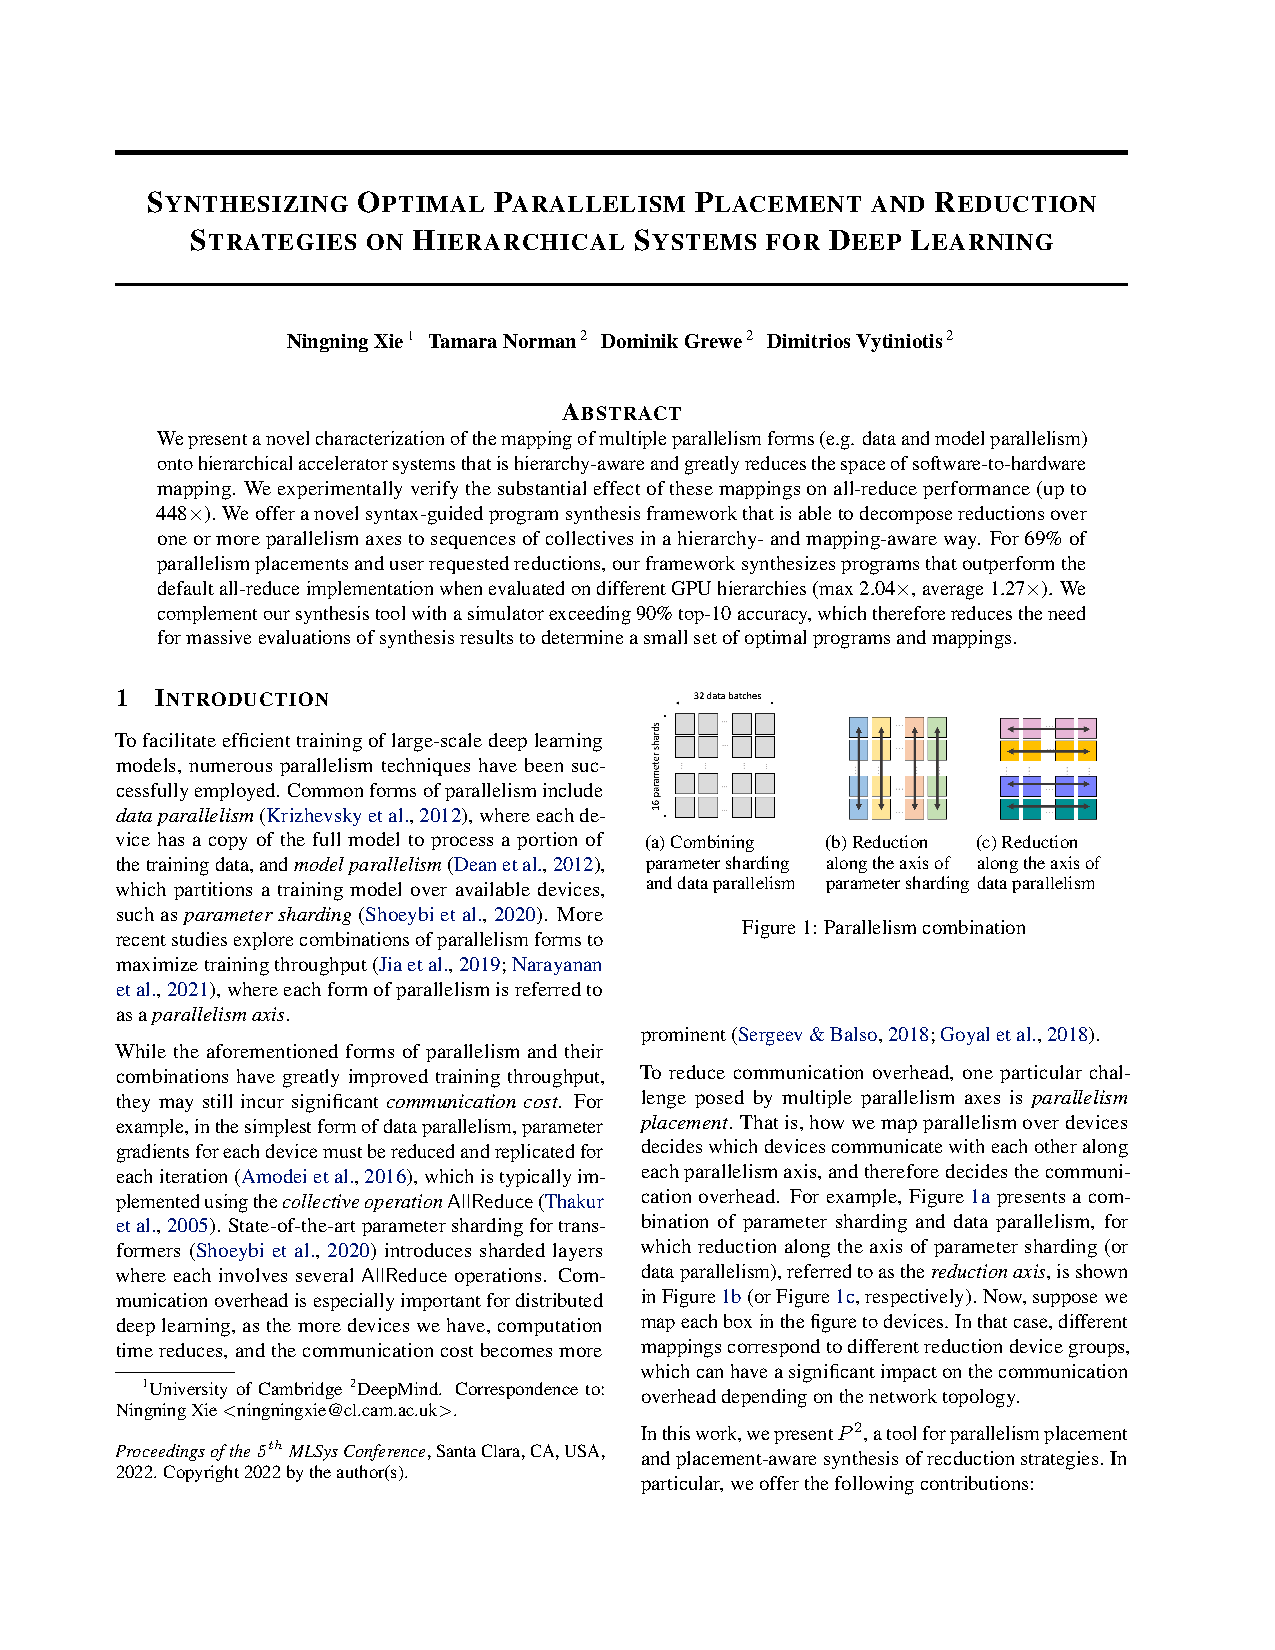
\includegraphics[page=1,trim=10.5cm 12.5cm 2.2cm 11.2cm,clip,scale=0.85]{p2.pdf}
    \end{frame}

    \begin{frame}
        \frametitle{Parallelism and Communication}

        \centering
        \includegraphics[page=2,trim=1.92cm 20cm 2.2cm 2.2cm,clip,scale=0.8]{p2.pdf}
    \end{frame}

    \begin{frame}
        \frametitle{$P^2$: a tool for parallelism placement and placement-aware synthesis of reduction strategies}

        \begin{itemize}
            \setlength{\itemsep}{.8em}
            \item Parallelism placement synthesis: mapping parallelism axes to the system hierarchy.
            \item Reduction strategy synthesis: synthesize a wide variety of reduction strategies to implement reductions using common collective operations.
        \end{itemize}
    \end{frame}


    \section{Design Overview}

    \begin{frame}
        \frametitle{Parallelism Placement}

        \textbf{Objective}: Deciding which parts of a partitioned program will execute on which parts of a system.
        \vskip 1em
        \textbf{Challenge}: Synthesizing all arbitrary device mappings can be extremely expensive.
        \vskip 1em
        \textbf{Solution}: Partition parallelism axes over the system hierarchy to generate topology-aware parallelism placements.
    \end{frame}

    \begin{frame}
        \frametitle{Parallelism Matrix}

        \centering
        \includegraphics[page=2,trim=1.92cm 20cm 2.2cm 2.2cm,clip,scale=0.8]{p2.pdf}
    \end{frame}

    \begin{frame}
        \frametitle{Reduction Strategy}

        $P^2$ synthesizes topology-aware reduction strategies using common collective operations.

        \vskip .5em
        \begin{itemize}
            \setlength{\itemsep}{.6em}
            \item (a) is commonly used but it does not utilize the topology of the system.
            \item (b) and (c) are strategies synthesized by $P^2$. Their first steps are within S0.
            \item (c) has fewer data to transfer over S1/S2 than (b), but it has more steps.
        \end{itemize}

        \vskip .5em
        \centering
        \includegraphics[page=3,trim=10.8cm 23.5cm 2cm 2.2cm,clip,scale=0.95]{p2.pdf}
    \end{frame}

    \begin{frame}
        \frametitle{Formalism of Collective Operations}

        Synthesizing all sequences of collective operations is not necessary. Some sequences of the operations lead to
        \textit{semantically invalid states} that can never reach the final desired state.

        \vskip 1em

        $P^2$ formalize common collective operations using Hoare triples. A Hoare triple
        $\{\mathcal{G}_1\}\mathcal{C}\{\mathcal{G}_2\}$ means when the precondition $\{\mathcal{G}_1\}$ is met,
        executing the command $\mathcal{C}$ establishes the postcondition $\{\mathcal{G}_2\}$.
    \end{frame}


    \section{Synthesis Algorithm}

    \begin{frame}
        \frametitle{Parallelism Placement}

        The Parallelism placement is defined by the parallelism matrix.

        \vskip 1.5em

        \centering
        \includegraphics[page=5,trim=1.9cm 12.8cm 11cm 10.7cm,clip,scale=0.95]{p2.pdf}
    \end{frame}

    \begin{frame}
        \frametitle{Collective Operations Notations and States}

        \begin{center}
            \vspace{-1em}
            \includegraphics[page=5,trim=1.9cm 4.9cm 11cm 20cm,clip,scale=0.95]{p2.pdf}
        \end{center}

        The state of a device is a $k \times k$ boolean matrix where $s[i][j] = 1$ means that device $j$ has contributed
        its original $i$th chunk to the reduction result.

        \vskip .5em
        \centering
        \includegraphics[page=5,trim=10.8cm 24cm 2cm 2.2cm,clip,scale=0.95]{p2.pdf}
    \end{frame}

    \begin{frame}
        \frametitle{Collective Operations Semantics}

        \vskip -.5em
        \centering
        \includegraphics[page=6,trim=1.92cm 17cm 2.2cm 2.2cm,clip,scale=0.8]{p2.pdf}
    \end{frame}

    \begin{frame}
        \frametitle{Reduction Program}

        A reduction strategy is represented as a \textit{program}, a list of reduction instructions.

        \begin{center}
            \includegraphics[page=6,trim=1.9cm 10.2cm 11cm 15.5cm,clip,scale=0.85]{p2.pdf}
        \end{center}

        \begin{columns}
            \begin{column}{0.55\textwidth}
                \includegraphics[page=7,trim=1.9cm 21cm 11.9cm 2.2cm,clip,scale=0.92]{p2.pdf}
            \end{column}
            \begin{column}{0.45\textwidth}
                \includegraphics[page=2,trim=2.2cm 22.8cm 14cm 2.4cm,clip,scale=0.95]{p2.pdf}
            \end{column}
        \end{columns}
    \end{frame}

    \begin{frame}
        \frametitle{Program Synthesis for Reduction Programs}

        The goal is to find a program $\mathcal{L}$ that

        \begin{center}
            \includegraphics[page=7,trim=10.8cm 12cm 2cm 14.2cm,clip,scale=0.85]{p2.pdf}
        \end{center}

        supposing $d_i$ reduces with devices $\bar{j}$.

        \vskip 1em

        $P^2$ uses a method called \textit{syntax-guided program synthesis} for this purpose.
    \end{frame}


    \section{Experiments}

    \begin{frame}
        \frametitle{Experimental Setup}

        \begin{columns}
            \begin{column}{0.5\textwidth}
                \begin{itemize}
                    \item 2 and 4 nodes on Google Cloud Platform.
                    \item 2 system topologies.
                \end{itemize}
            \end{column}
            \begin{column}{0.5\textwidth}
                \includegraphics[page=8,trim=1.9cm 18cm 11.4cm 2.2cm,clip,scale=0.8]{p2.pdf}
            \end{column}
        \end{columns}
    \end{frame}

    \begin{frame}
        \frametitle{Result 1}

        \textbf{The performance of AllReduce differs significantly among parallelism matrices, up to $448.5\times$.}

        \centering
        \includegraphics[page=8,trim=10.8cm 19.5cm 2cm 2.2cm,clip,scale=0.9]{p2.pdf}
    \end{frame}

    \begin{frame}
        \frametitle{Result 2}

        \textbf{The pruning techniques are effective for the synthesizer to achieve fast synthesis time.}

        \vskip 1em

        In the experiments, the program size limit is set to 5 for the synthesizer, which turns out to be sufficient to
        generate interesting reduction patterns. With this setup, the longest synthesis time is under 2 seconds (for up
        to 235 programs). Increasing the size limit makes the synthesis slightly slower, but, for most cases, does not
        generate new programs.
    \end{frame}

    \begin{frame}
        \frametitle{Result 3}

        \textbf{If the reduction axes can be put within one node, then a single step AllReduce inside that node is the most
        performant reduction due to fast local bandwidth.}
    \end{frame}

    \begin{frame}
        \frametitle{Result 4}

        \textbf{Synthesized programs can mitigate the impact of parallelism placement.}

        \vskip .5em
        \centering
        \includegraphics[page=9,trim=1.92cm 18cm 2.2cm 2.2cm,clip,scale=0.8]{p2.pdf}
    \end{frame}

    \begin{frame}
        \frametitle{Result 5}

        \textbf{For reduction across nodes, a topology-aware reduction program tends to outperform a single step
        AllReduce, with speedup on average $1.28\times$, upto $2.04\times$.}
    \end{frame}

    \begin{frame}
        \frametitle{Optimal strategies found by $P^2$}

        For ResNet-50 model, $P^2$ found the optimal strategy (ii) that achieves 15\% overall training time speedup
        compared to the baseline (Haiku).

        \centering
        \includegraphics[page=9,trim=10.8cm 14.5cm 2cm 11.2cm,clip,scale=1]{p2.pdf}
    \end{frame}


    \section{Summary}

    \begin{frame}
        \frametitle{Conclusion}

        \textbf{Strength}

        \vskip .6em
        \begin{itemize}
            \setlength{\itemsep}{.6em}
            \item Jointly optimize the parallelism placement and reduction strategy for hierarchical topologies.
            \item Formalize the collective semantics to automatically search for valid programs.
        \end{itemize}

        \vskip 1em
        \textbf{Limitation}

        \vskip .6em
        \begin{itemize}
            \setlength{\itemsep}{.6em}
            \item Only strictly symmetric and hierarchical topologies are considered.
            \item The optimal reduction strategy is simple and has already been studied.
            \item Why not take a step further and also consider the parallelism strategy?
        \end{itemize}
    \end{frame}

    \begin{frame}
        \frametitle{Takeaways}

        \begin{itemize}
            \setlength{\itemsep}{.8em}
            \item Operation synthesis
            \begin{itemize}
                \item Communication synthesis: transform a single collective operation into multiple smaller operations. ($P^2$, BlueConnect, SCCL, etc.)
                \item Computation synthesis: transform a computation operation into multiple smaller operations. (TASO, DietCode, etc.)
                \item Parallelism strategy synthesis: transform a computation operation into a series of communication and computation operations.
            \end{itemize}
            \item Define the state of the system and treat operations as directed links (with costs) that connect states.
        \end{itemize}
    \end{frame}

    \appendix

    \begin{frame}
        \vskip 1em

        \centering \huge
        Thank you!
    \end{frame}
\end{document}
